\documentclass{article}
\usepackage[x11names, svgnames, rgb]{xcolor}
\usepackage[utf8]{inputenc}
\usepackage{tikz}
\usetikzlibrary{snakes,arrows,shapes}
\usepackage{amsmath}
%
%

%

%

\begin{document}
\pagestyle{empty}
%
%
%

\enlargethispage{100cm}
% Start of code
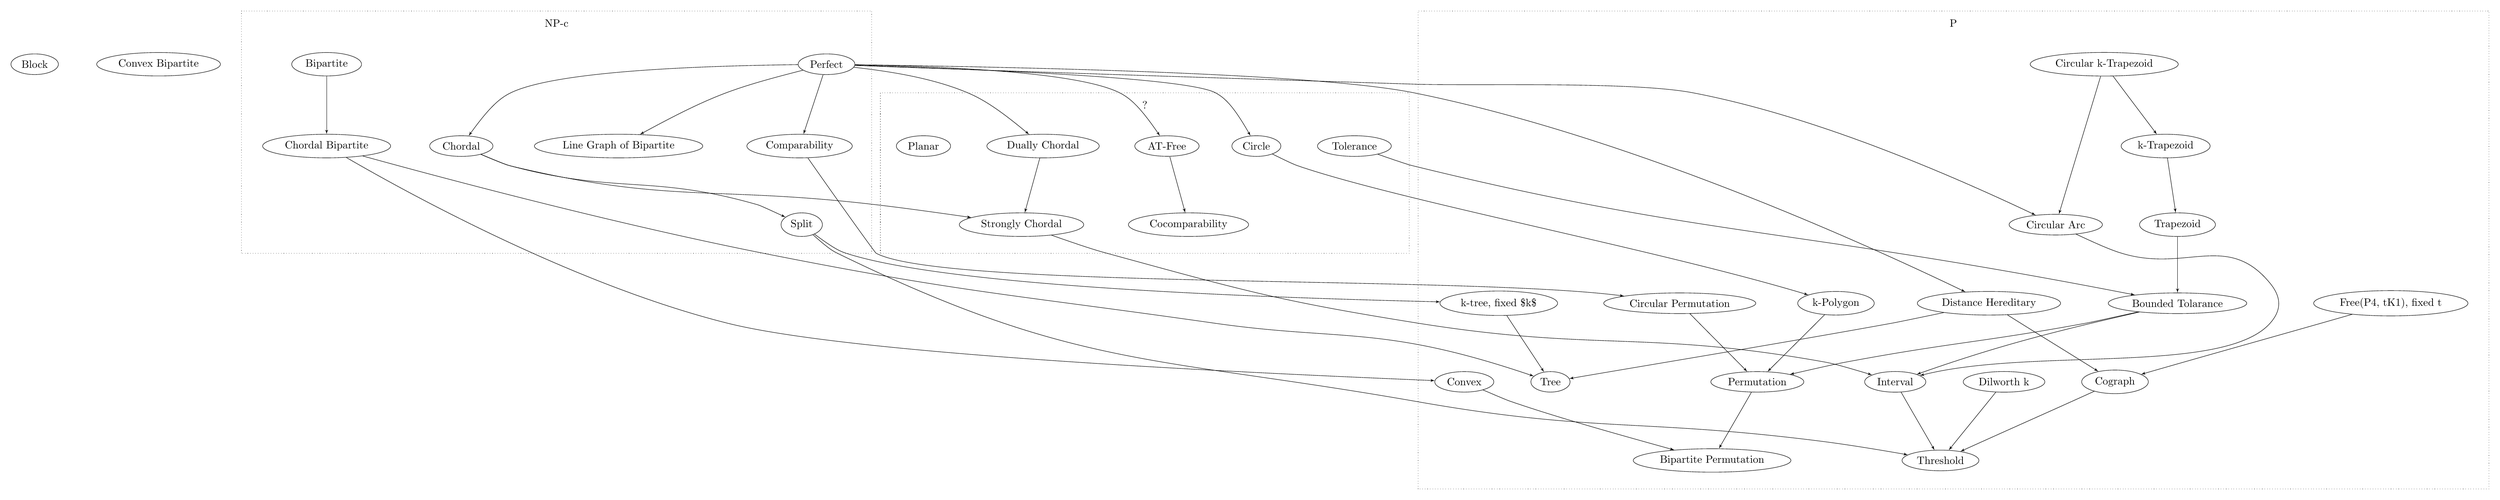
\begin{tikzpicture}[>=latex',line join=bevel,]
%%
\begin{scope}
  \pgfsetstrokecolor{black}
  \pgfsetdash{{\pgflinewidth}{2pt}}{0pt}
  \definecolor{strokecol}{rgb}{0.0,0.0,0.0};
  \pgfsetstrokecolor{strokecol}
  \draw [dotted] (220.0bp,227.0bp) -- (220.0bp,452.0bp) -- (805.0bp,452.0bp) -- (805.0bp,227.0bp) -- cycle;
  \draw (512.5bp,440.5bp) node {NP-c};
\end{scope}
\begin{scope}
  \pgfsetstrokecolor{black}
  \pgfsetdash{{\pgflinewidth}{2pt}}{0pt}
  \definecolor{strokecol}{rgb}{0.0,0.0,0.0};
  \pgfsetstrokecolor{strokecol}
  \draw [dotted] (1312.0bp,8.0bp) -- (1312.0bp,452.0bp) -- (2306.0bp,452.0bp) -- (2306.0bp,8.0bp) -- cycle;
  \draw (1809.0bp,440.5bp) node {P};
\end{scope}
\begin{scope}
  \pgfsetstrokecolor{black}
  \pgfsetdash{{\pgflinewidth}{2pt}}{0pt}
  \definecolor{strokecol}{rgb}{0.0,0.0,0.0};
  \pgfsetstrokecolor{strokecol}
  \draw [dotted] (813.0bp,227.0bp) -- (813.0bp,376.0bp) -- (1304.0bp,376.0bp) -- (1304.0bp,227.0bp) -- cycle;
  \draw (1058.5bp,364.5bp) node {?};
\end{scope}
  \node (LOB) at (570.0bp,326.5bp) [draw,ellipse] {Line Graph of Bipartite};
  \node (Perfect) at (763.0bp,402.5bp) [draw,ellipse] {Perfect};
  \node (Chordal) at (424.0bp,326.5bp) [draw,ellipse] {Chordal};
  \node (Comparability) at (738.0bp,326.5bp) [draw,ellipse] {Comparability};
  \node (Split) at (740.0bp,253.5bp) [draw,ellipse] {Split};
  \node (ChordalBipartite) at (299.0bp,326.5bp) [draw,ellipse] {Chordal Bipartite};
  \node (Bipartite) at (299.0bp,402.5bp) [draw,ellipse] {Bipartite};
  \node (Tree) at (1435.0bp,107.5bp) [draw,ellipse] {Tree};
  \node (Interval) at (1755.0bp,107.5bp) [draw,ellipse] {Interval};
  \node (Threshold) at (1797.0bp,34.5bp) [draw,ellipse] {Threshold};
  \node (CircularArc) at (1904.0bp,253.5bp) [draw,ellipse] {Circular Arc};
  \node (Permutation) at (1627.0bp,107.5bp) [draw,ellipse] {Permutation};
  \node (BipartitePermutation) at (1585.0bp,34.5bp) [draw,ellipse] {Bipartite Permutation};
  \node (CircularPermutation) at (1555.0bp,180.5bp) [draw,ellipse] {Circular Permutation};
  \node (Convex) at (1355.0bp,107.5bp) [draw,ellipse] {Convex};
  \node (KPolygon) at (1700.0bp,180.5bp) [draw,ellipse] {k-Polygon};
  \node (KTreeFixed) at (1387.0bp,180.5bp) [draw,ellipse] {k-tree, fixed \$k\$};
  \node (Cograph) at (1959.0bp,107.5bp) [draw,ellipse] {Cograph};
  \node (DilworthK) at (1856.0bp,107.5bp) [draw,ellipse] {Dilworth k};
  \node (P4tK1) at (2215.0bp,180.5bp) [draw,ellipse] {Free(P4, tK1), fixed t};
  \node (DistanceHereditary) at (1842.0bp,180.5bp) [draw,ellipse] {Distance Hereditary};
  \node (BoundedTolerance) at (2017.0bp,180.5bp) [draw,ellipse] {Bounded Tolarance};
  \node (Trapezoid) at (2017.0bp,253.5bp) [draw,ellipse] {Trapezoid};
  \node (KTrapezoid) at (2006.0bp,326.5bp) [draw,ellipse] {k-Trapezoid};
  \node (CircularKTrapezoid) at (1949.0bp,402.5bp) [draw,ellipse] {Circular k-Trapezoid};
  \node (Tolerance) at (1253.0bp,326.5bp) [draw,ellipse] {Tolerance};
  \node (ATFree) at (1079.0bp,326.5bp) [draw,ellipse] {AT-Free};
  \node (CComparability) at (1099.0bp,253.5bp) [draw,ellipse] {Cocomparability};
  \node (StronglyChordal) at (944.0bp,253.5bp) [draw,ellipse] {Strongly Chordal};
  \node (DuallyChordal) at (964.0bp,326.5bp) [draw,ellipse] {Dually Chordal};
  \node (Circle) at (1162.0bp,326.5bp) [draw,ellipse] {Circle};
  \node (Planar) at (853.0bp,326.5bp) [draw,ellipse] {Planar};
  \node (Block) at (28.0bp,402.5bp) [draw,ellipse] {Block};
  \node (ConvexBipartite) at (143.0bp,402.5bp) [draw,ellipse] {Convex Bipartite};
  \draw [->] (Perfect) ..controls (711.14bp,389.32bp) and (689.12bp,383.19bp)  .. (670.0bp,376.0bp) .. controls (649.85bp,368.43bp) and (628.27bp,358.24bp)  .. (LOB);
  \draw [->] (Perfect) ..controls (661.75bp,401.11bp) and (514.9bp,397.65bp)  .. (470.0bp,376.0bp) .. controls (459.12bp,370.75bp) and (449.48bp,361.75bp)  .. (Chordal);
  \draw [->] (Perfect) ..controls (754.17bp,375.37bp) and (750.4bp,364.2bp)  .. (Comparability);
  \draw [->] (Chordal) ..controls (463.81bp,309.75bp) and (466.94bp,308.81bp)  .. (470.0bp,308.0bp) .. controls (569.57bp,281.54bp) and (599.98bp,300.44bp)  .. (699.0bp,272.0bp) .. controls (700.44bp,271.59bp) and (701.9bp,271.13bp)  .. (Split);
  \draw [->] (Bipartite) ..controls (299.0bp,375.56bp) and (299.0bp,364.66bp)  .. (ChordalBipartite);
  \draw [->] (Interval) ..controls (1770.1bp,80.941bp) and (1776.2bp,70.697bp)  .. (Threshold);
  \draw [->] (CircularArc) ..controls (1949.3bp,232.34bp) and (1957.3bp,229.36bp)  .. (1965.0bp,227.0bp) .. controls (2024.8bp,208.62bp) and (2063.4bp,247.45bp)  .. (2103.0bp,199.0bp) .. controls (2113.4bp,186.27bp) and (2113.9bp,174.3bp)  .. (2103.0bp,162.0bp) .. controls (2060.0bp,113.53bp) and (1882.1bp,139.76bp)  .. (Interval);
  \draw [->] (Permutation) ..controls (1611.9bp,80.941bp) and (1605.8bp,70.697bp)  .. (BipartitePermutation);
  \draw [->] (CircularPermutation) ..controls (1581.4bp,153.42bp) and (1592.6bp,142.41bp)  .. (Permutation);
  \draw [->] (Convex) ..controls (1393.0bp,91.106bp) and (1396.0bp,90.01bp)  .. (1399.0bp,89.0bp) .. controls (1435.2bp,76.638bp) and (1475.9bp,64.697bp)  .. (BipartitePermutation);
  \draw [->] (KPolygon) ..controls (1673.2bp,153.42bp) and (1661.9bp,142.41bp)  .. (Permutation);
  \draw [->] (KTreeFixed) ..controls (1404.4bp,153.77bp) and (1411.5bp,143.27bp)  .. (Tree);
  \draw [->] (Cograph) ..controls (1897.7bp,79.643bp) and (1869.2bp,67.156bp)  .. (Threshold);
  \draw [->] (DilworthK) ..controls (1834.5bp,80.592bp) and (1825.5bp,69.84bp)  .. (Threshold);
  \draw [->] (P4tK1) ..controls (2108.9bp,150.06bp) and (2048.9bp,133.43bp)  .. (Cograph);
  \draw [->] (DistanceHereditary) ..controls (1758.0bp,163.1bp) and (1755.0bp,162.54bp)  .. (1752.0bp,162.0bp) .. controls (1651.0bp,143.66bp) and (1531.5bp,124.05bp)  .. (Tree);
  \draw [->] (DistanceHereditary) ..controls (1885.5bp,153.08bp) and (1905.0bp,141.26bp)  .. (Cograph);
  \draw [->] (BoundedTolerance) ..controls (1901.3bp,153.86bp) and (1852.8bp,141.81bp)  .. (Interval);
  \draw [->] (BoundedTolerance) ..controls (1937.4bp,163.0bp) and (1934.7bp,162.49bp)  .. (1932.0bp,162.0bp) .. controls (1833.7bp,143.92bp) and (1808.3bp,144.32bp)  .. (1710.0bp,126.0bp) .. controls (1703.4bp,124.77bp) and (1696.5bp,123.42bp)  .. (Permutation);
  \draw [->] (Trapezoid) ..controls (2017.0bp,227.29bp) and (2017.0bp,217.55bp)  .. (BoundedTolerance);
  \draw [->] (KTrapezoid) ..controls (2009.9bp,300.29bp) and (2011.4bp,290.55bp)  .. (Trapezoid);
  \draw [->] (CircularKTrapezoid) ..controls (1936.0bp,359.01bp) and (1921.4bp,311.35bp)  .. (CircularArc);
  \draw [->] (CircularKTrapezoid) ..controls (1969.5bp,374.9bp) and (1978.6bp,363.03bp)  .. (KTrapezoid);
  \draw [->] (ATFree) ..controls (1086.1bp,300.2bp) and (1088.9bp,290.34bp)  .. (CComparability);
  \draw [->] (DuallyChordal) ..controls (956.87bp,300.2bp) and (954.09bp,290.34bp)  .. (StronglyChordal);
  \draw [->] (Perfect) ..controls (882.94bp,397.6bp) and (1114.7bp,390.09bp)  .. (1308.0bp,384.0bp) .. controls (1365.6bp,382.19bp) and (1510.4bp,386.79bp)  .. (1567.0bp,376.0bp) .. controls (1675.4bp,355.33bp) and (1795.4bp,304.97bp)  .. (CircularArc);
  \draw [->] (Perfect) ..controls (900.4bp,400.28bp) and (1209.6bp,395.75bp)  .. (1308.0bp,376.0bp) .. controls (1496.7bp,338.13bp) and (1707.9bp,245.02bp)  .. (DistanceHereditary);
  \draw [->] (Perfect) ..controls (860.95bp,400.55bp) and (994.17bp,396.42bp)  .. (1035.0bp,376.0bp) .. controls (1045.6bp,370.7bp) and (1054.8bp,361.69bp)  .. (ATFree);
  \draw [->] (Perfect) ..controls (824.34bp,395.63bp) and (862.72bp,389.19bp)  .. (894.0bp,376.0bp) .. controls (908.94bp,369.7bp) and (923.93bp,359.89bp)  .. (DuallyChordal);
  \draw [->] (Perfect) ..controls (881.7bp,398.35bp) and (1095.6bp,391.09bp)  .. (1124.0bp,376.0bp) .. controls (1133.6bp,370.88bp) and (1141.6bp,362.14bp)  .. (Circle);
  \draw [->] (Chordal) ..controls (463.78bp,309.62bp) and (466.93bp,308.74bp)  .. (470.0bp,308.0bp) .. controls (617.36bp,272.77bp) and (658.53bp,289.74bp)  .. (809.0bp,272.0bp) .. controls (826.92bp,269.89bp) and (846.16bp,267.48bp)  .. (StronglyChordal);
  \draw [->] (ChordalBipartite) ..controls (441.07bp,287.39bp) and (581.93bp,251.27bp)  .. (704.0bp,227.0bp) .. controls (888.83bp,190.26bp) and (936.44bp,188.63bp)  .. (1123.0bp,162.0bp) .. controls (1242.2bp,144.98bp) and (1278.6bp,160.63bp)  .. (Tree);
  \draw [->] (ChordalBipartite) ..controls (390.08bp,273.63bp) and (536.9bp,195.68bp)  .. (671.0bp,162.0bp) .. controls (792.76bp,131.42bp) and (1177.8bp,114.93bp)  .. (Convex);
  \draw [->] (Comparability) ..controls (770.13bp,280.43bp) and (807.91bp,227.59bp)  .. (809.0bp,227.0bp) .. controls (870.77bp,193.69bp) and (1354.9bp,206.39bp)  .. (CircularPermutation);
  \draw [->] (Split) ..controls (768.87bp,232.03bp) and (774.94bp,228.98bp)  .. (781.0bp,227.0bp) .. controls (877.25bp,195.56bp) and (1169.9bp,185.69bp)  .. (KTreeFixed);
  \draw [->] (Split) ..controls (763.66bp,232.31bp) and (768.32bp,229.29bp)  .. (773.0bp,227.0bp) .. controls (995.2bp,118.49bp) and (1068.4bp,131.8bp)  .. (1312.0bp,89.0bp) .. controls (1474.3bp,60.481bp) and (1517.5bp,73.297bp)  .. (1681.0bp,53.0bp) .. controls (1701.2bp,50.49bp) and (1723.4bp,47.268bp)  .. (Threshold);
  \draw [->] (Tolerance) ..controls (1300.1bp,310.04bp) and (1304.1bp,308.95bp)  .. (1308.0bp,308.0bp) .. controls (1578.2bp,241.73bp) and (1653.7bp,251.37bp)  .. (BoundedTolerance);
  \draw [->] (StronglyChordal) ..controls (1003.8bp,232.5bp) and (1013.7bp,229.55bp)  .. (1023.0bp,227.0bp) .. controls (1150.0bp,192.3bp) and (1182.0bp,182.74bp)  .. (1312.0bp,162.0bp) .. controls (1478.2bp,135.48bp) and (1523.3bp,155.67bp)  .. (1689.0bp,126.0bp) .. controls (1695.3bp,124.88bp) and (1701.8bp,123.45bp)  .. (Interval);
  \draw [->] (Circle) ..controls (1194.7bp,310.27bp) and (1197.9bp,309.06bp)  .. (1201.0bp,308.0bp) .. controls (1294.9bp,275.79bp) and (1535.2bp,230.21bp)  .. (KPolygon);
%
\end{tikzpicture}
% End of code

%
\end{document}
%


